\documentclass{article}
\usepackage{tikz}

\begin{document}
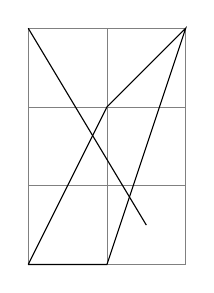
\begin{tikzpicture}
\draw[help lines] (0,0) grid (2,3);
\draw (0,0) -- (1,2)--(2,3)--(1,0)--(0,0);\draw (0,3) -- (1.5,0.5);
\end{tikzpicture}
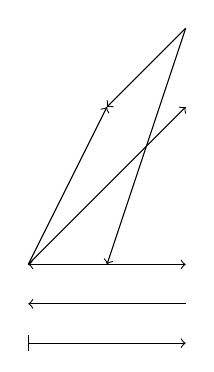
\begin{tikzpicture}
%\draw[help lines] (0,0) grid (2,3);
\draw [->] (0,0) --(2,2);
\draw [->](0,0) -- (1,2);
\draw [<-](1,2) --(2,3);
\draw [->](2,3)--(1,0);
\draw [->](1,0)--(0,0);
\draw [->] (0,0) -- (2,0);
\draw [<-] (0, -0.5) -- (2,-0.5);
\draw [|->] (0,-1) -- (2,-1);
\end{tikzpicture}
\begin{tikzpicture}
\draw [<->] (0,2) -- (0,0) -- (3,0);
\end{tikzpicture}


\begin{tikzpicture}
\draw [ultra thick] (0,1) -- (2,1);
\draw [thick] (0,0.5) -- (2,0.5);
\draw [thin] (0,0) -- (2,0);
\end{tikzpicture}
\end{document}